\documentclass{article}
\usepackage{graphicx} % Required for inserting images
\usepackage{amsfonts}
\usepackage{amsmath, amssymb}
\allowdisplaybreaks

\begin{document}
\begin{center} \huge Finding Outer Corners of the Cannon \\
\end{center}
Motivation: One way of changing the launch angle of the cannon is to click and hold the cannon and dragging the cannon up or down. However, when I was trying to create this code, I realised that the program took the cannon to only be the inside rectangular region. That is, if a user clicked on the border of the cannon, the program did not recognise this as a successful click on the cannon. So, the following method lets us find the outer corners of the cannon, given the inner corners of the cannon. \vspace{\baselineskip}\\
\textbf{Important Note}
\indent To match the coordinate system followed by HTML and JavaScript, right and downwards are considered to be positive directions. That is, a point $M$ that is to the right of a point $N$ will have a larger $x$ coordinate and a point $M$ that is below a point $N$ will have a larger $y$ coordinate.\vspace{\baselineskip}\\
Consider the following diagram:\\
\begin{figure}[h]
	\centering
	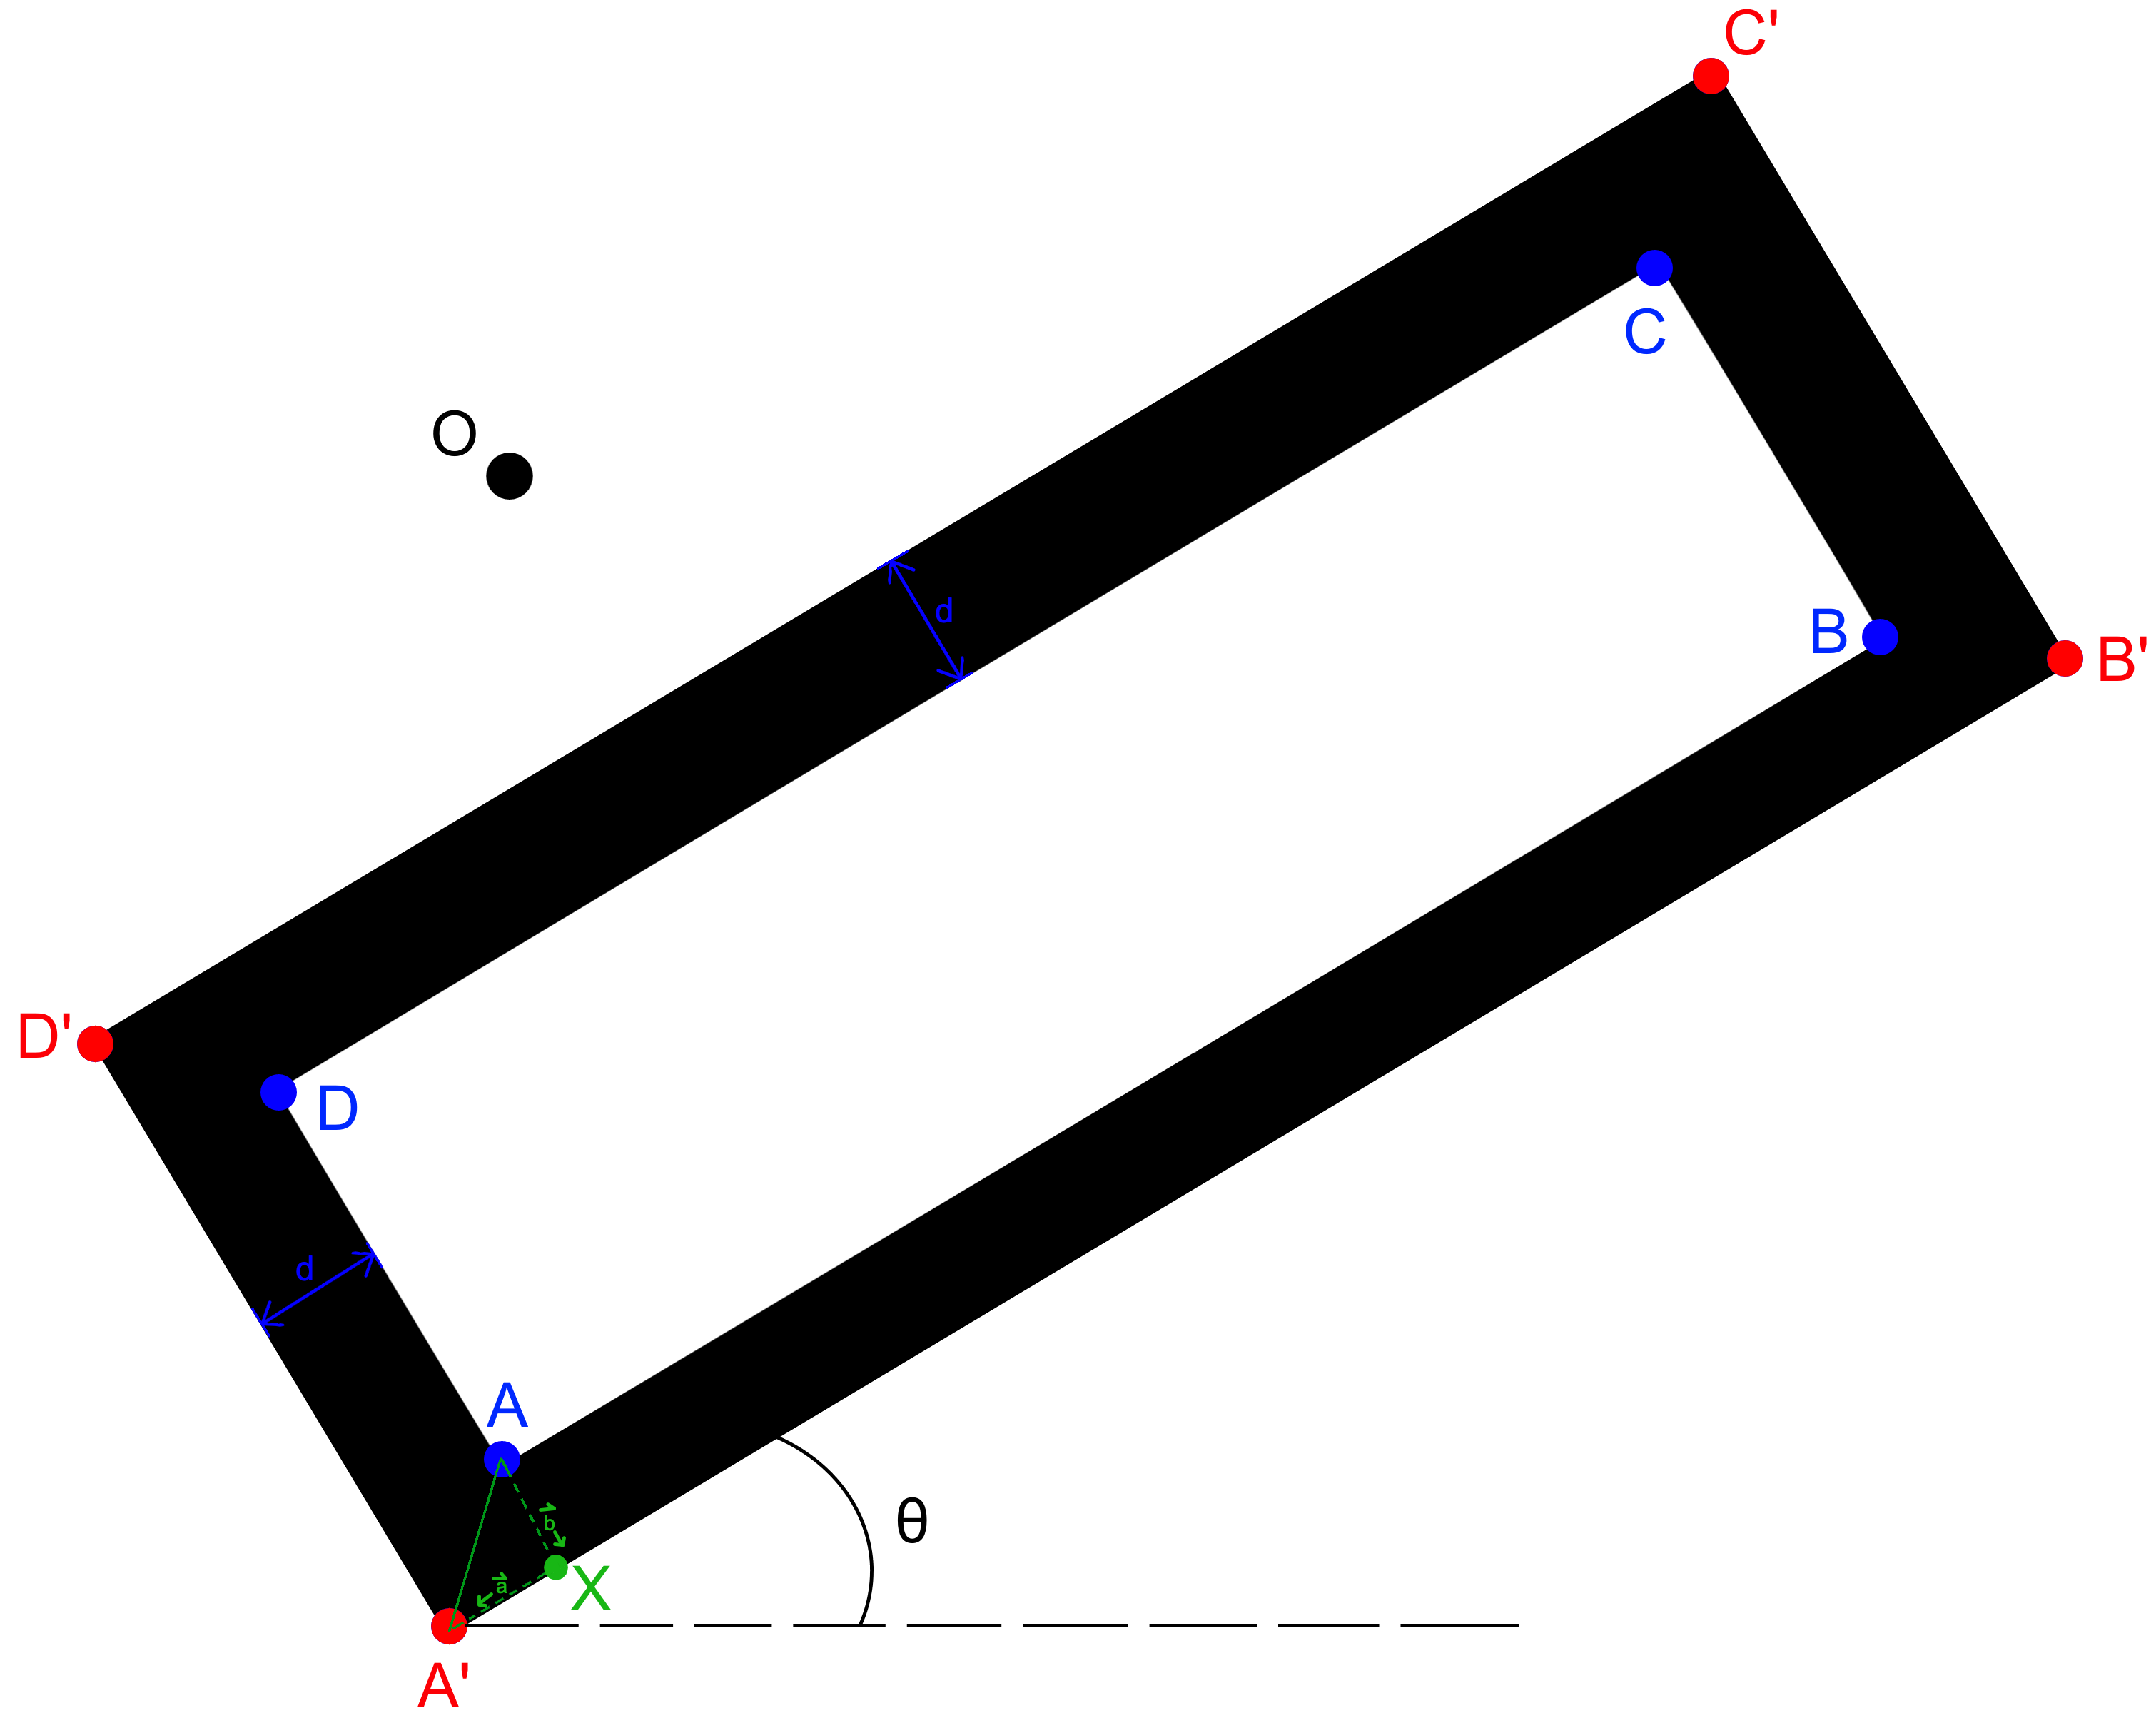
\includegraphics[scale=0.08]{Images/FindingOuterCornersOfCannon_1.png}
	\caption{Overview of the whole cannon}
\end{figure}\\
Recall that points $A$, $B$, $C$ and $D$ are known points, while $A'$, $B'$, $C'$ and $D'$ are the points we are looking for.\vspace{\baselineskip}\\
Point $X$ is constructed such that $AX \perp A'X$. Let $$\vec{a} = \overrightarrow{XA'}$$ and $$\vec{b} = \overrightarrow{AX}.$$ Notice that $\overrightarrow{AA'} = \vec{b} + \vec{a}$. Since the thickness of the border is constant at any region we can define $$d = |\vec{a}| = |\vec{b}|.$$
\vspace{\baselineskip}\\
Consider the following diagram:\\
\begin{figure}[h]
	\centering
	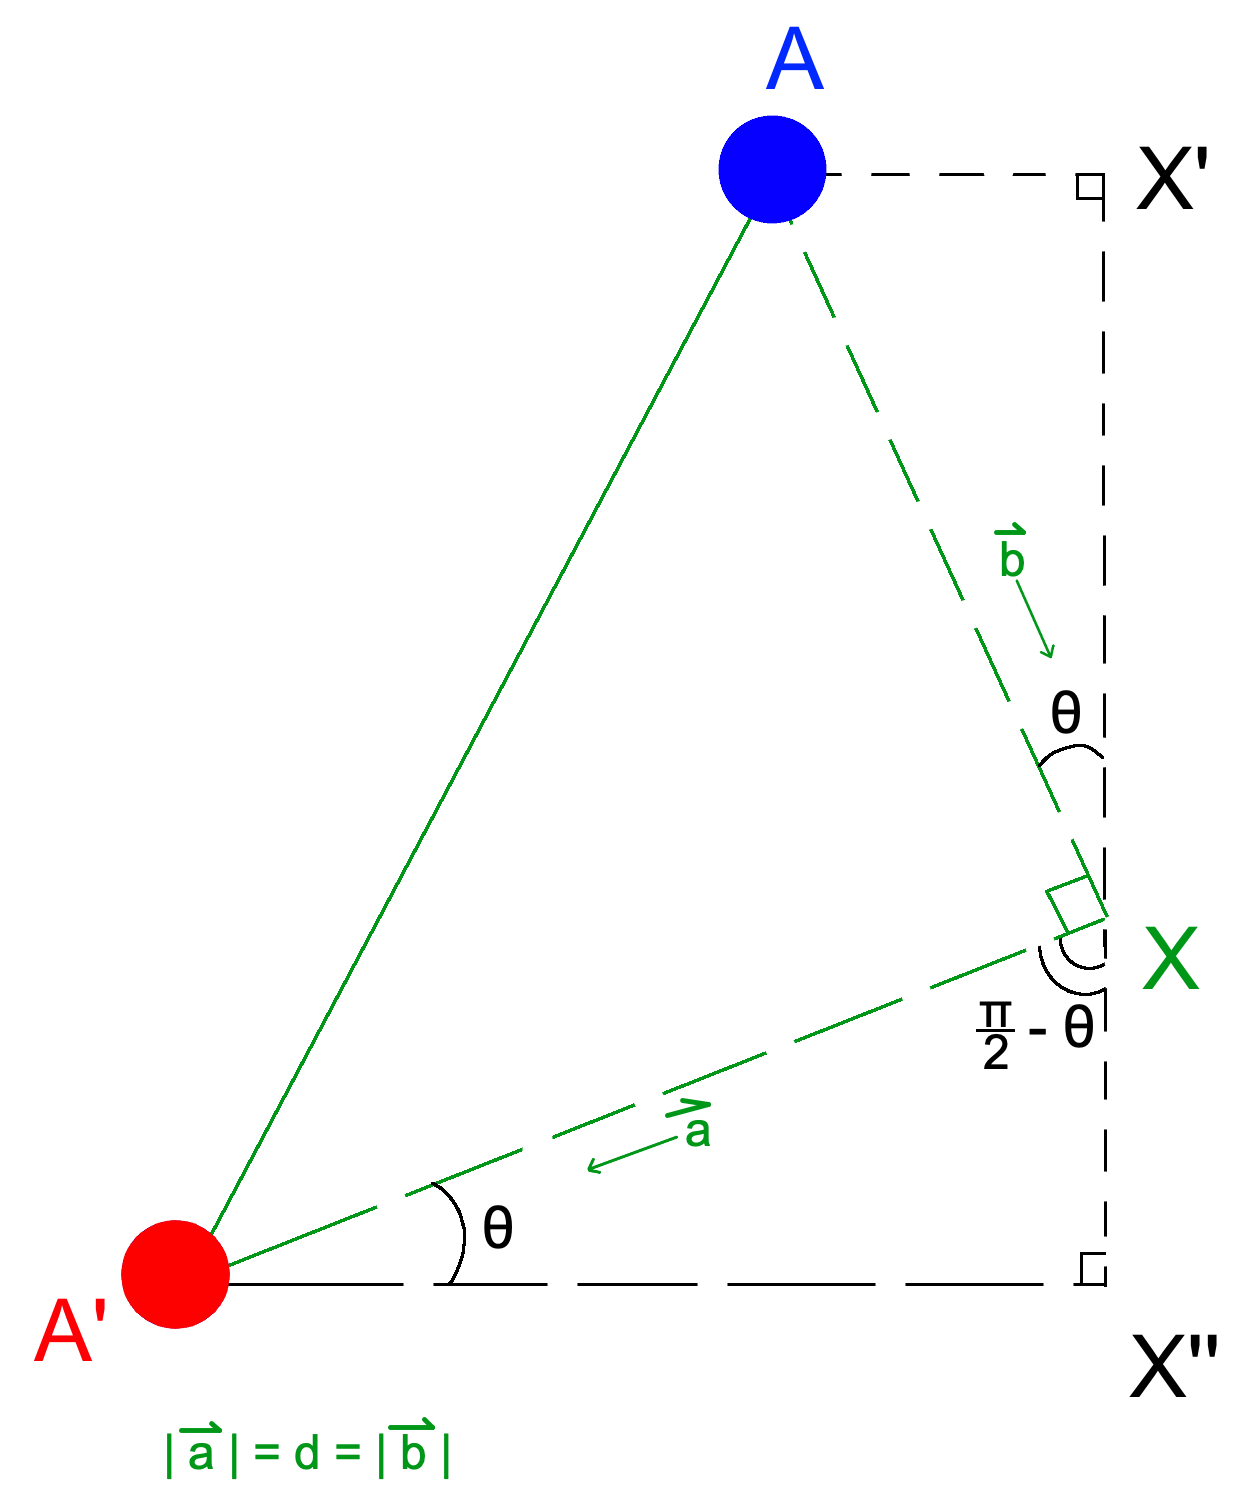
\includegraphics[scale=0.2]{Images/FindingOuterCornersOfCannon_2.png}\\
	\caption{Focusing on the point A'}
\end{figure}\\
Notice that $\angle XA'X'' = \theta$ since $A'X''$ is a horizontal line and $A'X$ represents a segment of the long edge of the cannon. Therefore, $\angle A'XX'' = \frac{\pi}{2} - \theta$ by the internal angle sum of a triangle and $\angle AXX' = \theta$ by the angle of a straight line. \vspace{\baselineskip}\\
Breaking $\vec{a}$ and $\vec{b}$ into their horizontal and vertical components, 
$$\overrightarrow{XX''} = 
\begin{pmatrix}
	0\\
	d\sin{\theta}
\end{pmatrix}$$
and
$$\overrightarrow{X''A'} =
\begin{pmatrix}
	-d\cos{\theta}\\
	0
\end{pmatrix},$$ 
while 
$$\overrightarrow{AX'} = 
\begin{pmatrix}
	d\sin{\theta}\\
	0\\
\end{pmatrix}$$
and 
$$\overrightarrow{X'X} = 
\begin{pmatrix}
	0\\
	d\cos{\theta}
\end{pmatrix}.$$
Therefore, we can conclude that $$\vec{a} = \overrightarrow{XX''} + \overrightarrow{X''A'}= 
\begin{pmatrix}
	-d\cos{\theta}\\
	d\sin{\theta}
\end{pmatrix}$$
and 
$$\vec{b} = \overrightarrow{AX'} + \overrightarrow{X'X} = 
\begin{pmatrix}
	d\sin{\theta}\\
	d\cos{\theta}
\end{pmatrix}.$$
Now considering Figure 1 again, we can find the position vectors of $A'$, $B'$, $C'$ and $D'$. $$\overrightarrow{OA'} = \overrightarrow{OA} + \vec{b} + \vec{a},$$ $$\overrightarrow{OB'} = \overrightarrow{OB} + \vec{b} - \vec{a},$$ $$\overrightarrow{OC'} = \overrightarrow{OC} -\vec{b} - \vec{a}$$ and $$\overrightarrow{OD'} = \overrightarrow{OD} - \vec{b} + \vec{a}.$$

\end{document}
